\chapter{Data Analysis}

\section{Efficiencies}
\paragraph{}The High resolution spectrometers are capable of detecting a myriad of particles that track through the detectors. The designed of an experimental trigger uses the properties of the individual detectors to capture data of the meaningful events. Many accidentals, back ground, and unwanted events trigger the data acquisition system. The removal of these unwanted events take place during analysis via software cuts. Restricting the applicable signal from certain detectors through different cuts allows for the rejection of back ground particles and prevents contamination in the yield extraction. 

\subsection{Particle Identification Efficiency}
One of the largest sources of contamination for the MARATHON experiment is negatively charge pions. These pions are removed through software cuts made in the total signal from the ten cherenkov PMTs(photomultiplier tubes) and the energy deposited into the blocks of both layers of the calorimeter. Electrons can be identified by their behavior in the spectrometer. High quality electrons will track through the entire detector stack to deposit most of their energy into the total calorimeter system and creating a large amount of light in the cherenkov. Though this knowledge tight cuts can be used to study the efficency of the particle identification system. Plotting the signal in the cherenkov versus the energy deposited into both layers of the calorimeter allow for visual representation of the sampling cuts made in the efficiency studies. Figure \ref{elesample}, 



\begin{figure}[h]
{\centering
\textbf{Particle ID for the two layers of the calorimeter and the cherenkov}\par\medskip}

\label{Prl1Plr2}
\includegraphics[width=5cm]{Lprl1}
\includegraphics[width=5cm]{Lprl2}
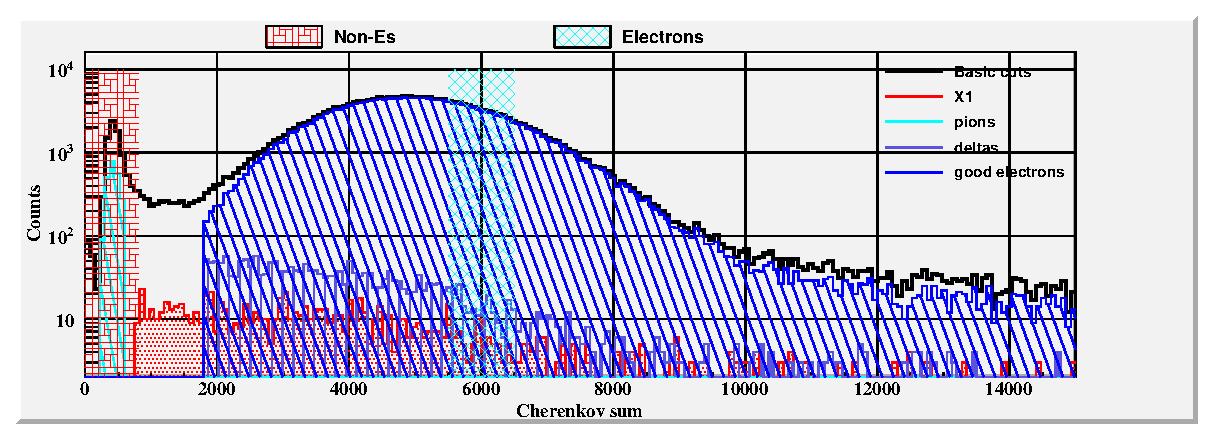
\includegraphics[width=5cm]{Lcerasum}
\caption{Electrons and other back ground particles identified via cuts in the total calorimeter and the gas cherenkov shown in the individual layers of the calorimeters.}
\end{figure}

